
\section{Modelo de Dados}
\label{sec:modelo_de_dados}

A modelagem de dados foi realizada com o intuito de representar os dados utilizados pelo \emph{webscan}
da maneira mais abstrata possível, sem se preocupar com locais ou métodos de armazenamento.
Para modelar a aplicação foi utilizado o diagrama de entidade-relacionamento (Figura \ref{fig:der},
que faz parte da metodologia do Modelo Entidade-Relacionamento). 

\subsection{Diagrama Entidade-Relacionamento}
\begin{figure}[ht]
 \centering
  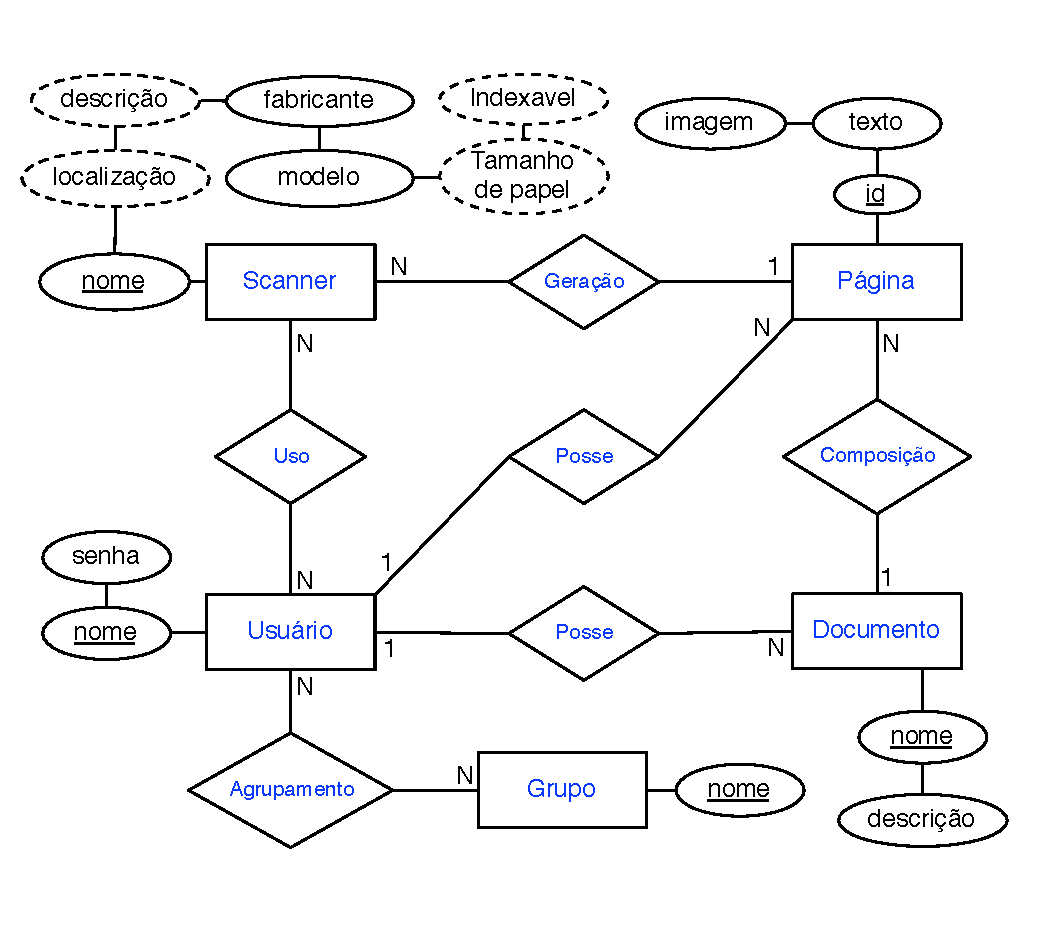
\includegraphics[scale=0.75]{img/der.pdf}
  \caption {Diagrama entidade-relacionamento}
  \label{fig:der}
\end{figure}
